\documentclass[../HAFiscal]{subfiles}
\begin{document}

\subsection{Estimation of the "splurge" factor}	

We define splurging as the free spending of available income without concern for intertemporal maximization of utility. As we will show in this section, a model allowing for splurging performs well at capturing the shorter and longer term response of consumption to income shocks. Specifically, we show that our model can account well for the results of \citet{fagereng_mpc_2021}, who study the impact of lottery winnings in Norway on consumption using millions of datapoints from the Norwegian population registry. To do so we calibrate our model to reflect the Norwegian economy and estimate the splurge factor, as well as the distribution of discount factors in the population to match two empirical moments. 	
	
First, we match the steady-state distribution of liquid wealth in the model to its empirical counterpart. Due to the lack of data on the liquid wealth distribution in Norway, we resort to the corresponding data from the US - assuming that liquid wealth inequality is comparable across these countries. Specifically, we impose as targets the cummulative liquid wealth share at the 20th, 40th, 60th and 80th income percentile, which equal 0\%, 0.4\%, 2.5\% and 11.7\%.\footnote{@Edmund, where is this data from?} Hence, 87.3\% of the total liquid wealth is  held by the top income quintile. The data is plotted in figure \ref{fig:liquwealthdistribution}.
Second, we take from \citet{fagereng_mpc_2021} the marginal propensity to consume out of a one-period income shock. We not only target the contemporaneous respone of consumption to the income shock, but also the subsequent impact on consumption in years one to four after the income shock. The share of lottery winnings expended at different time horizions, as found in \citet{fagereng_mpc_2021}, are plotted in figure \ref{fig:aggmpclotterywin}.


\begin{figure}[htb]
	\centering
	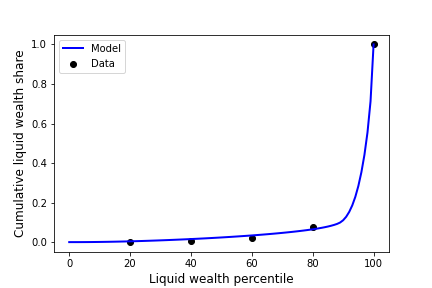
\includegraphics[width=0.8\linewidth]{../Code/HA-Models/Target_AggMPCX_LiquWealth/Figures/LiquWealth_Distribution}
	\caption{Distribution of liquid wealth}
	\label{fig:liquwealthdistribution}
\end{figure}

\begin{figure}[htb]
	\centering
	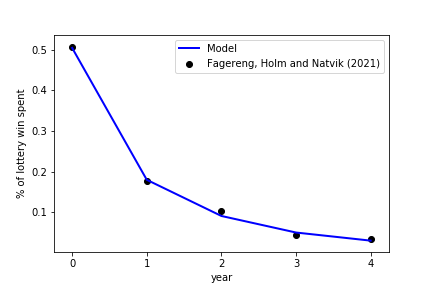
\includegraphics[width=0.8\linewidth]{../Code/HA-Models/Target_AggMPCX_LiquWealth/Figures/AggMPC_LotteryWin}
	\caption{Share of lottery win spent}
	\label{fig:aggmpclotterywin}
\end{figure}



The remaining model parameters are calibrated to reflect the Norwegian economy. Specifically, we set the real interest rate to 2\% annually and the unemployment rate to 4.4\%, in line with \citet{aursland_state-dependent_2020}. The quartarly probability to survive is calibrated to $1-1/160$, reflecting an expected working life of 40 years. Aggregate productivity growth is set to 1\% annually following \citet{kravik_navigating_2019}. The unemployment net replacement rate is calibrated to 60\% following \citet{oecd_net_2020}. Finally, we set the real interest rate on liquid debt to 13.6\% and the borrowing constraint on 80\% of permanent income following data from the Norwegian debt registry \citet{gjeldsregistret_nokkeltall_2022}.\footnote{Specifically, we determine the average volume-weighted interest rate on liquid debt, which consists of consumer loans, credit and payment card debt and all other unsecured debt. To determine the borrowing limit on liquid debt we determine the ratio between total credit card limit divided by total wage income in Norway. We use data from December 2019.} The standard deviation of the permanent and transitory shock are 0.07 and 0.346, respectively. [@Hakon, could you add a few sentences on the data on which the std was estimated?]

Using the calibrated model, unexpected lottery winnings are simulated and the share of the lottery spent in each year is calculated. Specifically, each simulated agent receives a lottery win in a random quarter of the first year of the simulation. The size of the lottery win is itself random and spans the range of lottery sizes found in \citet{fagereng_mpc_2021}. The estimation procedure minimizes the distance between the targets and model moments by selecting the splurge factor and the distribution of discount factors in the population, where the latter are assumed to be uniformly distributed in the range $[\beta-\nabla, \beta+\nabla]$. We approximate the uniform distribution of discount factors with a discrete approximation and let the population consist of $7$ different discount types.

The estimation yields a splurge factor of 0.32 and a distribution of discount factors described by $\beta = 0.986$ and a $\nabla=0.0174$. Given these estimated parameters and the remaining calibrated ones, the model is able to replicate the time path of consumption in response to a lottery win from \citet{fagereng_mpc_2021} and the targeted distribution of liquid wealth very well, see figure \ref{fig:splurge_estimation}.

\end{document}	

